%%%%%%%%%%%%%%%%%%%%%%%%%%%%%%%%%%%%%%%%%
% Journal Article
% LaTeX Template
% Version 1.4 (15/5/16)
%
% This template has been downloaded from:
% http://www.LaTeXTemplates.com
%
% Original author:
% Frits Wenneker (http://www.howtotex.com) with extensive modifications by
% Vel (vel@LaTeXTemplates.com)
%
% License:
% CC BY-NC-SA 3.0 (http://creativecommons.org/licenses/by-nc-sa/3.0/)
%
%%%%%%%%%%%%%%%%%%%%%%%%%%%%%%%%%%%%%%%%%

%----------------------------------------------------------------------------------------
%	PACKAGES AND OTHER DOCUMENT CONFIGURATIONS
%----------------------------------------------------------------------------------------

\documentclass[twoside,twocolumn]{article}

\usepackage{graphicx}
\usepackage{siunitx}

\usepackage{blindtext} % Package to generate dummy text throughout this template 

\usepackage[sc]{mathpazo} % Use the Palatino font
\usepackage[T1]{fontenc} % Use 8-bit encoding that has 256 glyphs
\linespread{1.05} % Line spacing - Palatino needs more space between lines
\usepackage{microtype} % Slightly tweak font spacing for aesthetics

\usepackage[english]{babel} % Language hyphenation and typographical rules

\usepackage[hmarginratio=1:1,top=32mm,columnsep=20pt]{geometry} % Document margins
\usepackage[hang, small,labelfont=bf,up,textfont=it,up]{caption} % Custom captions under/above floats in tables or figures
\usepackage{booktabs} % Horizontal rules in tables

\usepackage{lettrine} % The lettrine is the first enlarged letter at the beginning of the text

\usepackage{enumitem} % Customized lists
\setlist[itemize]{noitemsep} % Make itemize lists more compact

\usepackage{abstract} % Allows abstract customization
\renewcommand{\abstractnamefont}{\normalfont\bfseries} % Set the "Abstract" text to bold
\renewcommand{\abstracttextfont}{\normalfont\small\itshape} % Set the abstract itself to small italic text

\usepackage{titlesec} % Allows customization of titles
\renewcommand\thesection{\Roman{section}} % Roman numerals for the sections
\renewcommand\thesubsection{\roman{subsection}} % roman numerals for subsections
\titleformat{\section}[block]{\large\scshape\centering}{\thesection.}{1em}{} % Change the look of the section titles
\titleformat{\subsection}[block]{\large}{\thesubsection.}{1em}{} % Change the look of the section titles

\usepackage{fancyhdr} % Headers and footers
\pagestyle{fancy} % All pages have headers and footers
\fancyhead{} % Blank out the default header
\fancyfoot{} % Blank out the default footer
\fancyhead[C]{UC Berkeley Transactions on Advanced Digital Integrated Circuits $\bullet$ \today} % Custom header text
\fancyfoot[RO,LE]{\thepage} % Custom footer text

\usepackage{titling} % Customizing the title section

\usepackage{hyperref} % For hyperlinks in the PDF

% USER PACKAGES
\usepackage[backend=biber, sorting=none, giveninits=true, bibencoding=utf8]{biblatex}
\addbibresource{final_report.bib}
\renewcommand*{\bibfont}{\small}

%----------------------------------------------------------------------------------------
%	TITLE SECTION
%----------------------------------------------------------------------------------------

\setlength{\droptitle}{-4\baselineskip} % Move the title up

\pretitle{\begin{center}\Huge\bfseries} % Article title formatting
\posttitle{\end{center}} % Article title closing formatting
\title{rFPGA: A dense, efficient NEMS-CMOS FPGA Architecture} % Article title
\author{%
\textsc{Lars Tatum}\\[1ex] % Your name
\normalsize University of California \\ % Your institution
\normalsize \href{mailto:lpt@berkeley.edu}{lpt@berkeley.edu} % Your email address
\and % Uncomment if 2 authors are required, duplicate these 4 lines if more
\textsc{Erik Anderson}\\[1ex] % Second author's name
\normalsize University of California \\ % Your institution
\normalsize \href{mailto:efa@eecs.berkeley.edu}{efa@eecs.berkeley.edu} % Second author's email address
}
\date{\today} % Leave empty to omit a date
\renewcommand{\maketitlehookd}{%
\begin{abstract}
\noindent FPGAs, like all reconfigurable systems, exhibit significantly
worse performance than their ASIC counterparts. This disparity is primarily due
to the extremely flexible yet power-hungry and physically large programmable routing
network inside the FPGA. To alleviate this problem, several versions of CMOS compatible 
Back-End-Of-Line (BEOL) mechanical relays have been proposed to create denser 
and more efficient programmable interconnects. In this paper, we analyze the area benefits of 
a relay based FPGA (rFPGA) with respect to the traditional CMOS-only FPGA, 
and lay the groundwork for future power/performance analysis. 
Our designs will use ASAP7 \cite{clark_asap7_2016}, 
a predictive 7nm PDK, to realistically gauge the benefits and drawbacks of rFPGAs 
in the modern semiconductor landscape.
\end{abstract}
}

%----------------------------------------------------------------------------------------

\begin{document}

% Print the title
\maketitle

%----------------------------------------------------------------------------------------
%	ARTICLE CONTENTS
%----------------------------------------------------------------------------------------

\section{Introduction}

Field Programmable Gate Arrays (FPGAs) have long been used to enable rapid prototyping of digital systems pre-tapeout of Application Specific Integrated Circuits (ASICs)\cite{8187326}. The framework they provide for high-performance reconfigurable digital systems is now proving useful for end-use applications including ML-acceleration, cryptocurrency mining, high-frequency stock trading, and software-defined radios. FPGA demand is predicted to continue rising as these prototyping and end-use markets increase in demand.

To enable this flexibility, FPGA-based systems are much more demanding than their ASIC counterparts. FPGAs come with larger die area requirements, increased delay, and high dynamic and static power consumption. These factors increase the cost of FPGA-based systems and lower their potential performance over ASIC-based systems. Recently, CMOS compatible devices have been developed that could mitigate these area/power/performance drawbacks.  Nano-Electro-Mechanical-Systems (NEMS) provide a promising, easily-integrable way to further FPGA-based systems. But first, a look at where all this overhead comes from in FPGAs.

\subsection{The Island-Style FPGA architecture}

FPGAs general consist of a general logic fabric as well as application-specific components, such as block RAM, DSPs, clocking, and I/O blocks\cite{8187326}. This project will tackle the general logic fabric, since it makes up the majority of the FPGA.

SRAM-based island-style FPGAs represent the vast majority of commercial and academic
FPGA implementations \cite{farooq_fpga_2012}. Fig. \ref{fig:island} shows an example of a simplified island-style FPGA. 
To create an island-style FPGA a basic \textit{tile} must first be constructed. Each tile consists of one 
\textit{configurable logic block} (CLB), two \textit{connection boxes} (CBs), and one \textit{switch box} (SB). 
The CLB contains N basic logic elements (BLEs) which each contain a K-input look-up-table (LUT) and a flip-flop. 
CLBs are used to implement arbitrary combinational and sequential logic circuits. 
Each CLB can be programmed to perform an arithmetic or state-based portion of a larger logic system. CLBs are connected together using reconfigurable interconnects. In addition, CLBs provide an intra-cluster routing network to connect the CLB I/O to the individual BLE I/O. Reconfigurable Interconnects, made up of Connection Blocks and Switch Boxes, are the "breadboard" of the FPGA. They allow the portions of the digital system to communicate. The CBs connect the CLBs to their adjacent routing channels, while the SBs provide the connections
between intersecting routing channels. It is common to fold the output portion of 
the CBs into the SB \cite{chen_efficient_2010}. Thus, the same MUXes used for
connecting routing channels can be enlarged to accomodate the additional 
CLB output connections. The tile's routing configuration is stored in a configuration SRAM array
and shifted out to configuration registers at the beginning of normal operation. Working within
the constraints of ASAP7, the SRAM was implemented as an array of flip flops.

\begin{figure}[!hbt]
    \centering
    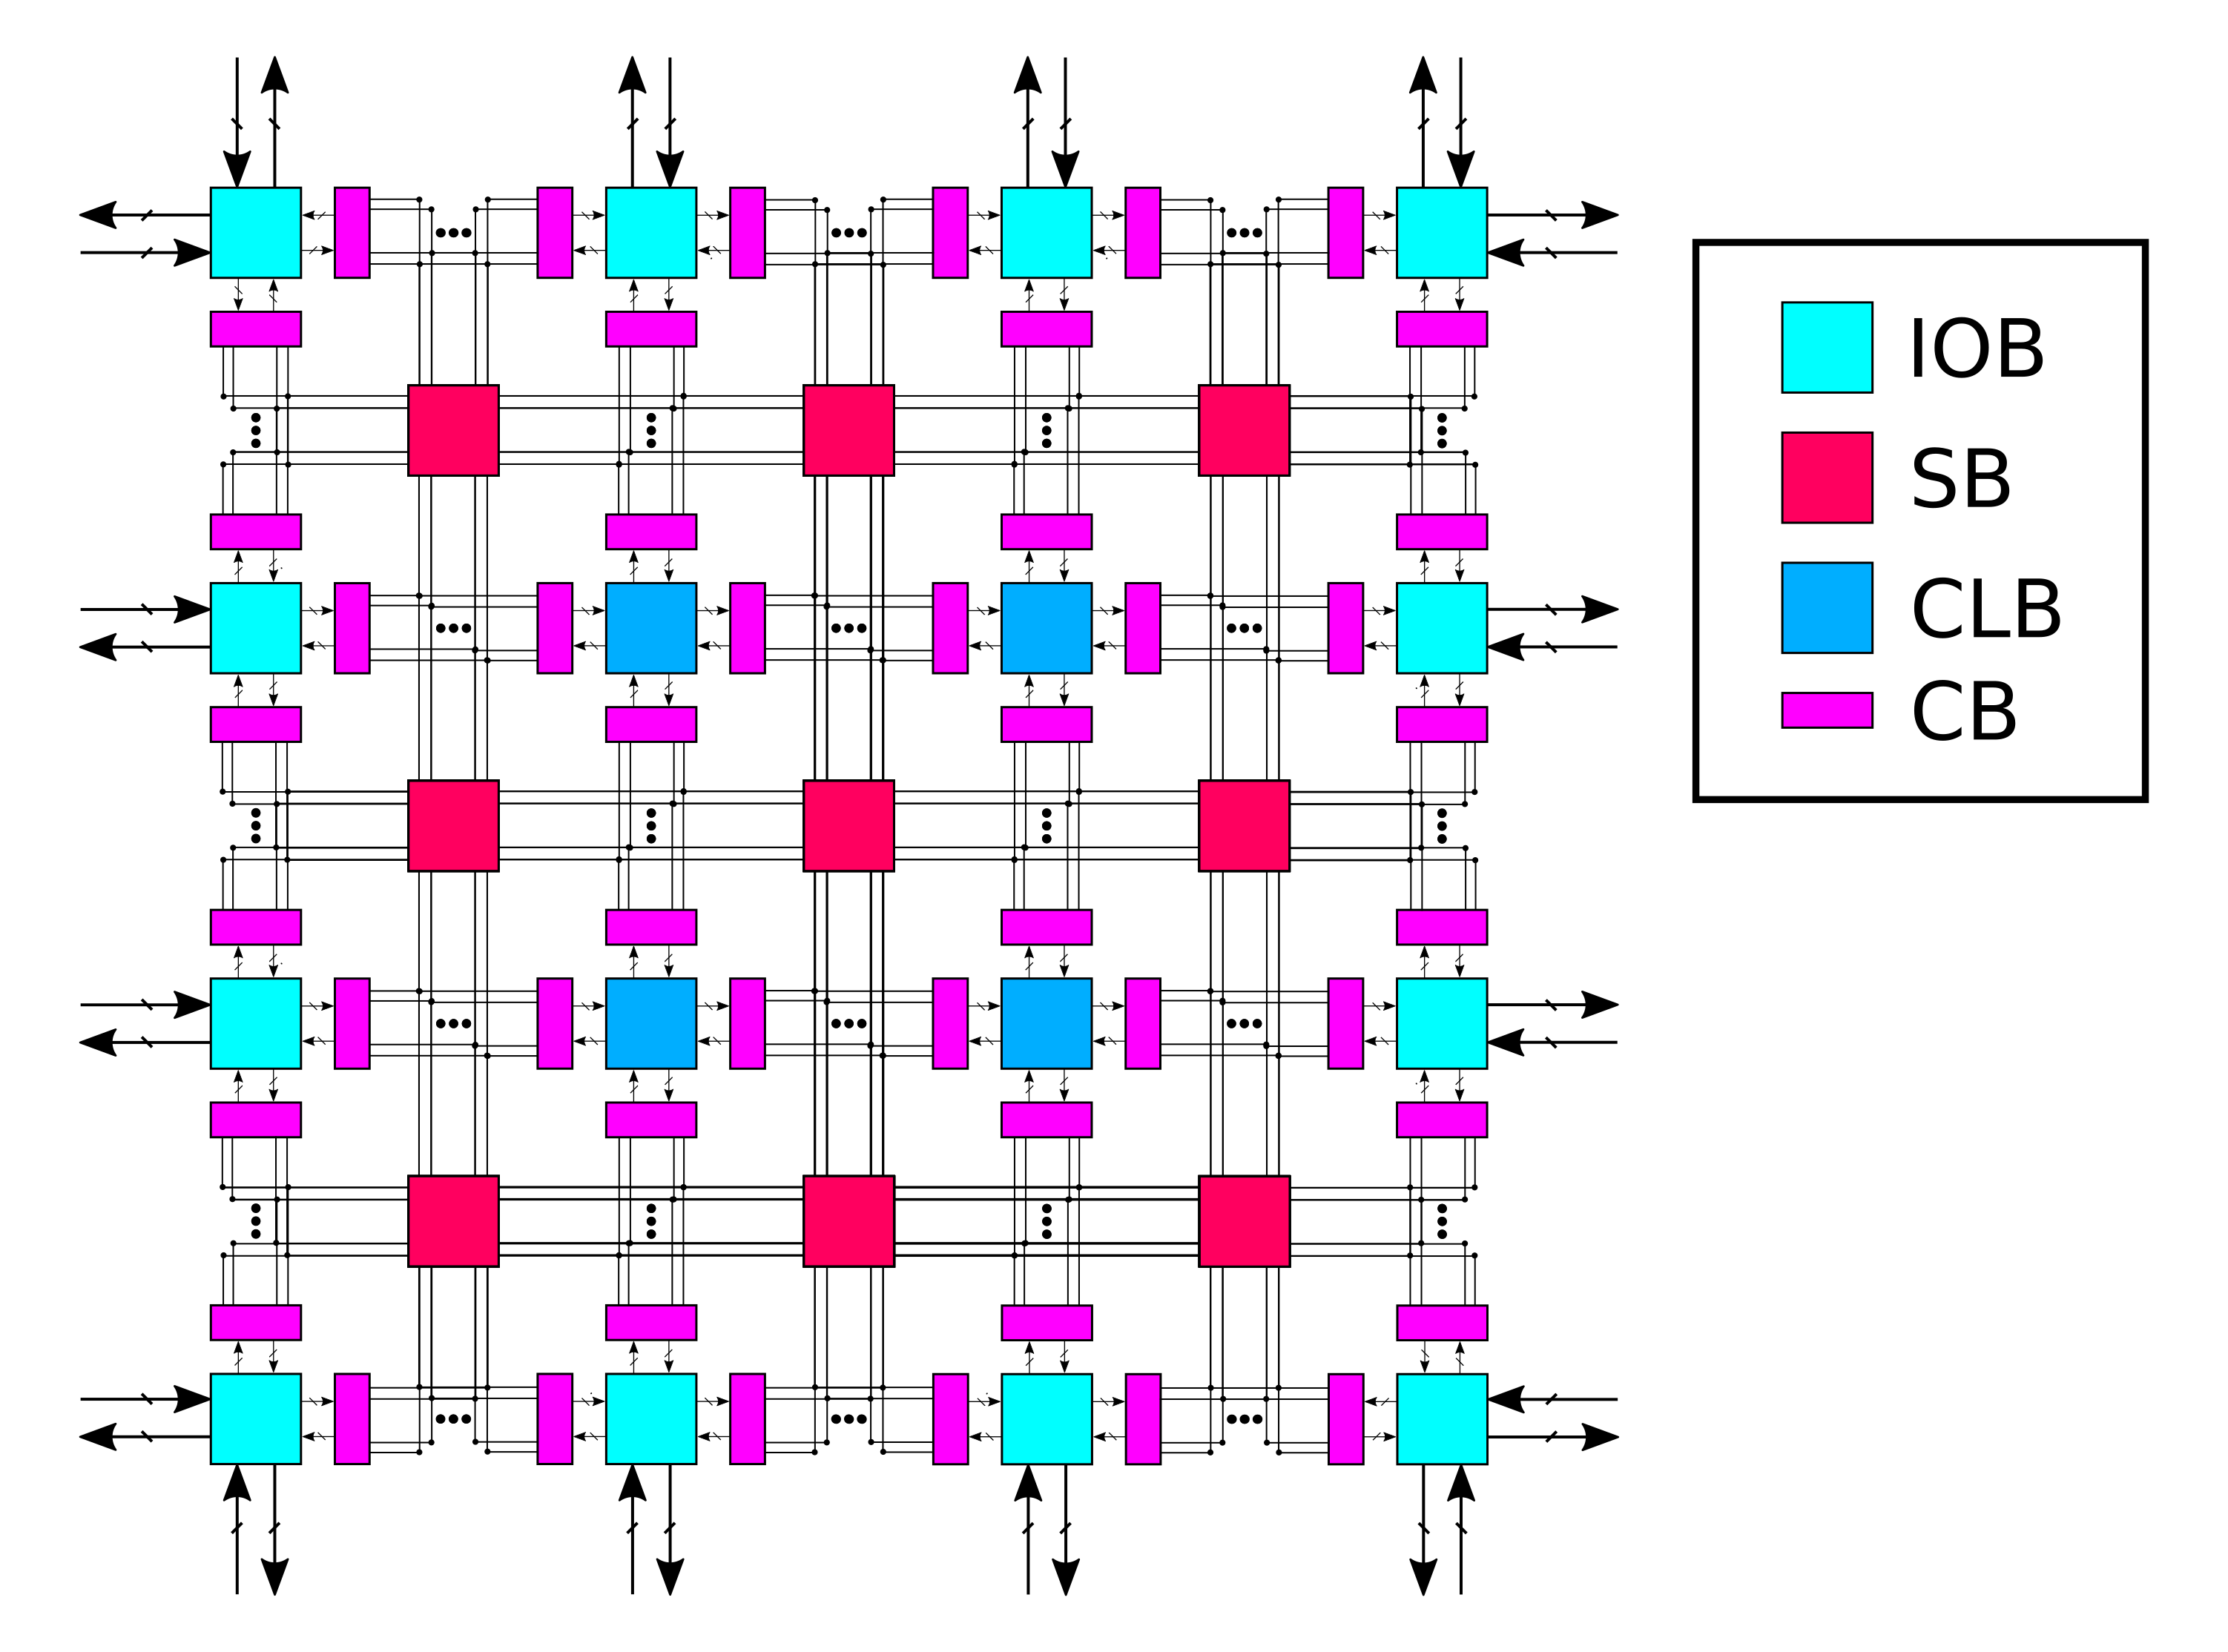
\includegraphics[width=0.5\textwidth]{figs/island_style.png}
    \caption{Basic island style FPGA}
    \label{fig:island}    
\end{figure}

These Reconfigurable Interconnects dominate the area/power overhead incurred by FPGAs \cite{ALTERA}. In an ASIC, interconnects are simple, passive elements; circuits are connected using fixed metal lines paths above the transistor devices. To enable design flexibility, FPGAs add SRAM configuration storage as well as the mux circuitry required to connect blocks and wires. Not only does this additional circuitry incur a large power/delay overhead, it also must be implemented completely in the Front-End-Of-Line alongside logic transistors, adding significantly to die area.

What if these power/performance/area drawbacks could be mitigated to enhance FPGA-based systems? ASIC circuits are connected solely via Back-End-Of-Line (BEOL) Metal lines. If FPGAs could emulate this structure, much of the overhead incurred from reconfigurable interconnects could be eliminated.

\subsection{NEM Relays}

Nanoelectromechanical Relays are electrically actuated mechanical switches. Notably, they experience zero leakage, have the potential for lower on-state resistance than NMOS pass gate, and can be implemented in the BEOL in a CMOS-compatible process flow\cite{LIU}. The major disadvantages of NEM relays are large mechanical switching delay (> 1ns)\cite{chen_integrated_2008} and lower reliability with respect to transistors ($10^9$ - $10^{10}$ cycles). Two prominent relay device architectures are lateral "crab style" relays and vertical interconnect relays. Due to their hysteretic properties, they can be implemented to replace both the interconnect pass-gates and their corresponding SRAM cells.

The lateral "crab-style" relays are the result of many years of development at Stanford and UC Berkeley to create an efficient CMOS compatible NEM relay\cite{LIU}. These relays are switched on/off using the gate to body voltage difference. When "off", no current flows across the air gap. When "on", current flows between the drain and source with low on-state resistance. With this design, the device can be body-biased to have an extremely small switching voltage, experimentally shown to be sub-50mV range.

The vertical relays are designed to be more compact and compatible with existing CMOS process flows. Rather than using deposited metal or polysilicon as the structural material, these vertical relays use the already-present metal vias/interconnects in a CMOS process flow\cite{SIKDER}. These relays can be implemented as single-pole double-throw switches or simpler single-pole single-throw switches \cite{OLDSIKDER} (like the lateral relays). Both have their own drawbacks and benefits. While the lateral relays involve a "custom" structure, these vertical ones can be designed within the constraints of standard CMOS BEOL design rules as an ASIMPS process; i.e, they use standard metal line/via structures, and dimensions are standard for the process node. Due to this, we explore the vertical relay implementation in depth.

%------------------------------------------------

\section{Methods}\label{sec:methods}
The aforementioned island-style architecture will be used to construct two functionally equivalent FPGAs using CMOS and NEMS routing schemes.

% Describe specific FPGA architecture that we will use 
To ensure that our results are consistent with previous works, we
will create a very similar tile to the one described in \cite{chen_efficient_2010}. 
This tile consists of 10 4-LUT BLEs w/ 22 input pins and 10 output pins.
In order to simplify the design, the CBs in our tile will connect both
the outputs and inputs of the CLB to the adjacent routing channel.
The intra-CLB routing network will be fully populated, allowing for connection 
between any BLE input and CLB input as well as between any BLE output and CLB output.
The SB flexibility will be set to 3 ($f_{SB} = 3$), allowing all 
incoming signals to the SB to be switched left, right, or straight through. 
The CB input and output flexibilities will be set to 0.2 ($f_{CB-in} = 0.2$) 
and 0.1 respectively ($f_{CB-out} = 0.1$). These flexibilities determine the 
proportion of signals within the adjacent routing channels that the CB can 
connect an input or output signal to. The channel width will be set to 104 wires
($W=104$) with 80 of those wires representing the minimum channel width for 
CLBs with 10 outputs and length 4 routing segments ($W_{min} = 2 * 10 * 4 = 80$).


The Princeton Reconfigurable Field Programmable Array generator (pRGA) 
was used to create the RTL description of this architecture.
pRGA allows a user to specify an architecture description and 
generates the corresponding verilog using python. A quirk of 
pRGA is that the default configuration system implemented is 
a very long bitstream scan-chain that extends through the LUTs 
and interconnect configuration network. To more accurately baseline 
state-of-the-art SRAM-based CMOS FPGAs, the interconnect configuration 
was stored in an SRAM-register combo, while the LUTs were still scan chain based.

% Detail CMOS implementation (mainly mux architecture) 
The CMOS FPGA will serve as a baseline for the NEMS design.
Because the programmable interconnect (PI) will be replaced with NEM relays, the make up
of our baseline's PI will significantly impact the perceived benefits. 
CMOS transmission gates show promise for scaled nodes, and were used to build the MUXes used 
for the PI and the LUTs. Note that semi-recent commercial FPGAs continue to use pass-transistors with gate-boosting and internal buffering
to achieve a slightly lower area-delay product. \cite{chiasson_should_2013}.

% Detail how we will model the NEMs relays

\subsection{Relay Integration}
In Connection Blocks and Switch Boxes, a combination of muxes and buffers are used to route Logic Blocks to wires and different routing wires together. Traditional CMOS muxes are implemented as two or more-stage serial pass transistor structures for minimum area-delay product. For the relay based designs, these NMOS pass transistors (and corresponding configuration SRAM cells) are replaced with NEM relays. To reduce the number of series relays as well as the number of total relays, a one-stage NEM-based mux is preferable for reduced area and delay\cite{chen_efficient_2010}.

NEM relay based routing muxes can eliminate the need for configuration SRAM by implementing a CMOS half-select programming scheme\cite{chen_efficient_2010}. Similar to the half-select scheme of crossbar arrays, the relays are partitioned into an array of row and column lines for programming. The relay states are preserved by a constant holding voltage on the row lines and constant select voltage on the column lines. During configuration, an additional (positive or negative) select voltage is superimposed on on the row lines "to be programmed", and the column lines are grounded. This voltage is just enough to actuate the relay into the desired state, but not so much that catastrophic pull-in occurs. Since relays have no leakage current, the only power required to keep the relays in the "hold state" is the dynamic power used during configuration to charge the parasitic capacitance. Since state-of-the-art FPGAs consist of thousands of tiles, the half-select programming array is predicted to consume <5\% of total die area.

The NEMs relays can be modeled as simple RC circuits when configured in the 
ON-state \cite{chen_efficient_2010} \cite{chen_integrated_2008} and can be ignored, 
because they are physically disconnected from the 
circuit, when in the OFF-state. Modeling the dynamics of the NEMs relays
as they switch on and off is not as important as the steady-state behavior
for this analysis. Switching time will only affect the FPGA configuration
time, and thus as long as the relays are not prohibitively slow, which they
have been shown not to be \cite{chen_integrated_2008}, then the dynamics of the switches can be 
ignored for our purposes.

% %UPDATE WITH REAL FIGURE INFO
% \begin{figure}[!hbt]
%     \centering
%     \caption{RC Circuit Model of "ON" relay}
%     \label{fig:methods}
%     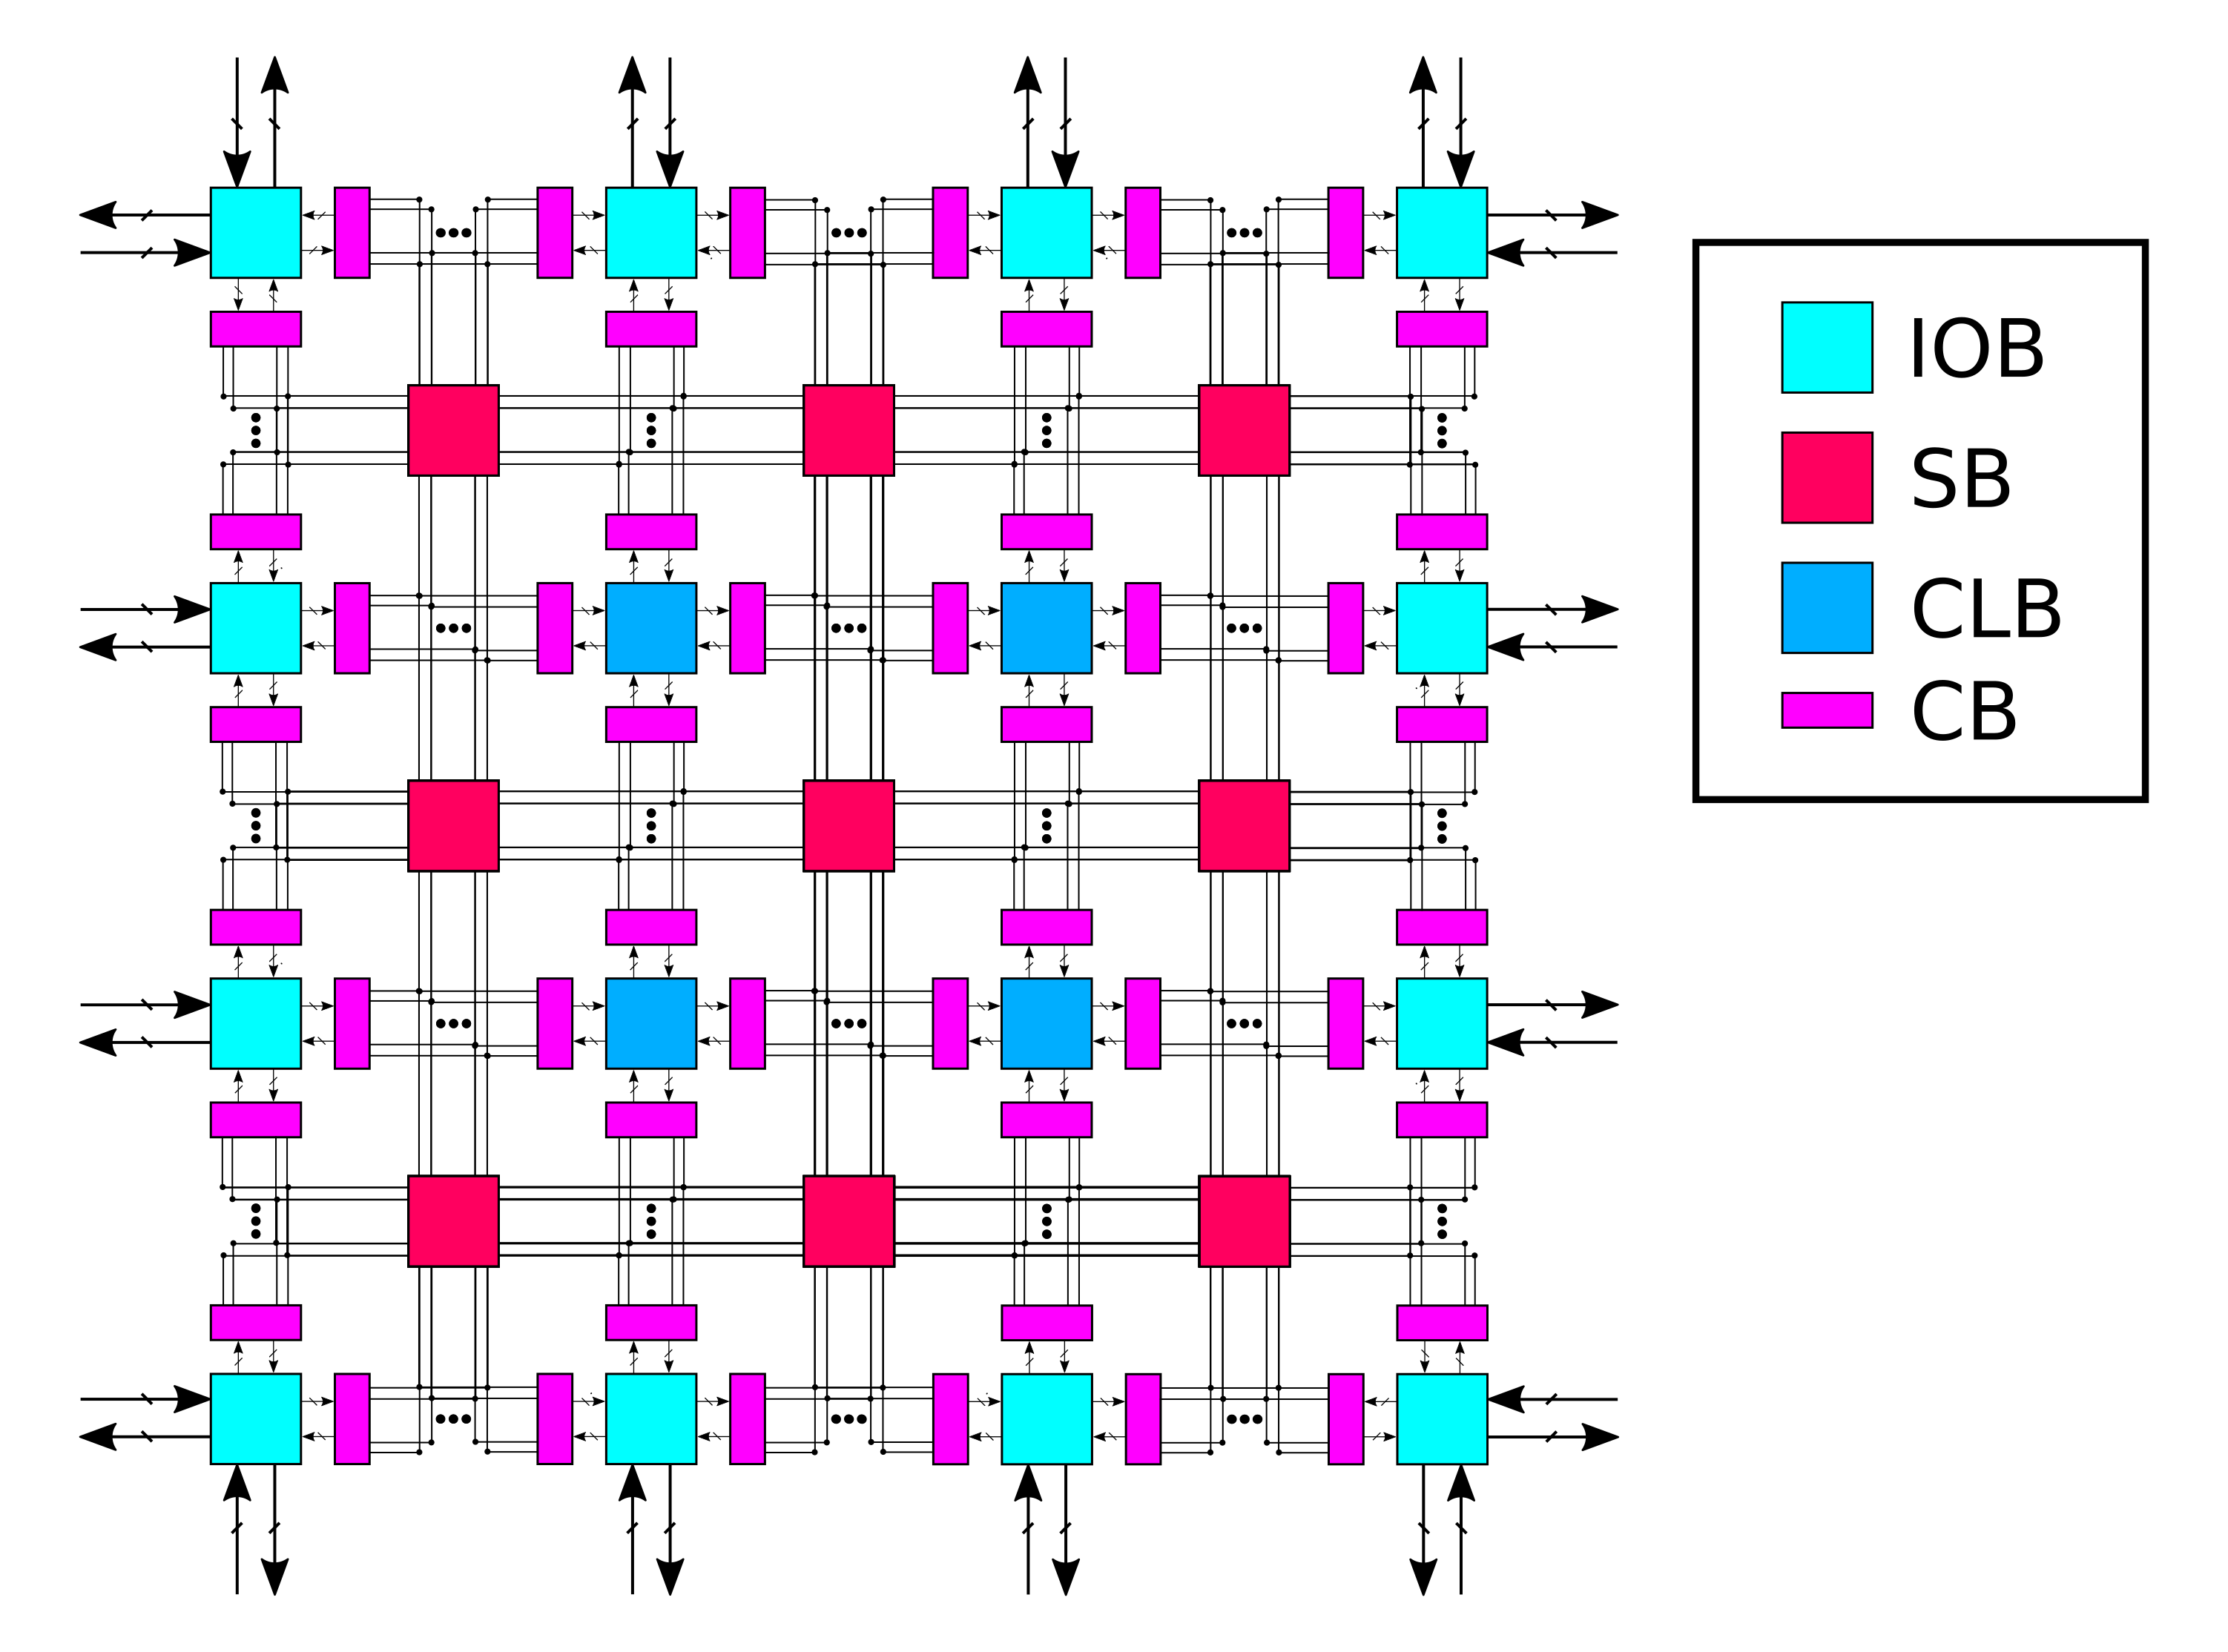
\includegraphics[width=0.5\textwidth]{figs/island_style.png}
% \end{figure}

% Detail how we will P&R the NEMs relays
For design Place And Route, the structure from \cite{OLDSIKDER} was implemented "as-is" with the simulated relay design parameters and resultant optimal dimensions. The contact gap is 20nm, and the actuation gap is 60nm. The metal beam is 75nm x 18nm. These result in a total switch area footprint of 75nm x 96nm, or 0.0072 square microns.
Note for sake of consistency with the referenced work, this design does not conform to ASAP7 design rules. For example, the upper metal layers are thinner than the minimum metal length, and the metal gaps have not been vetted.
It shoud also be noted that any fabrication-assistive structures required to create the NEM relay structure have been omitted. Many times, metal "masking layers" and upper metal layer keepout boundaries must be implemented to prevent unintentional destruction of other standard CMOS structures during the anisotropic release etch.

%UPDATE WITH REAL FIGURE INFO
\begin{figure}[!hbt]
    \centering
    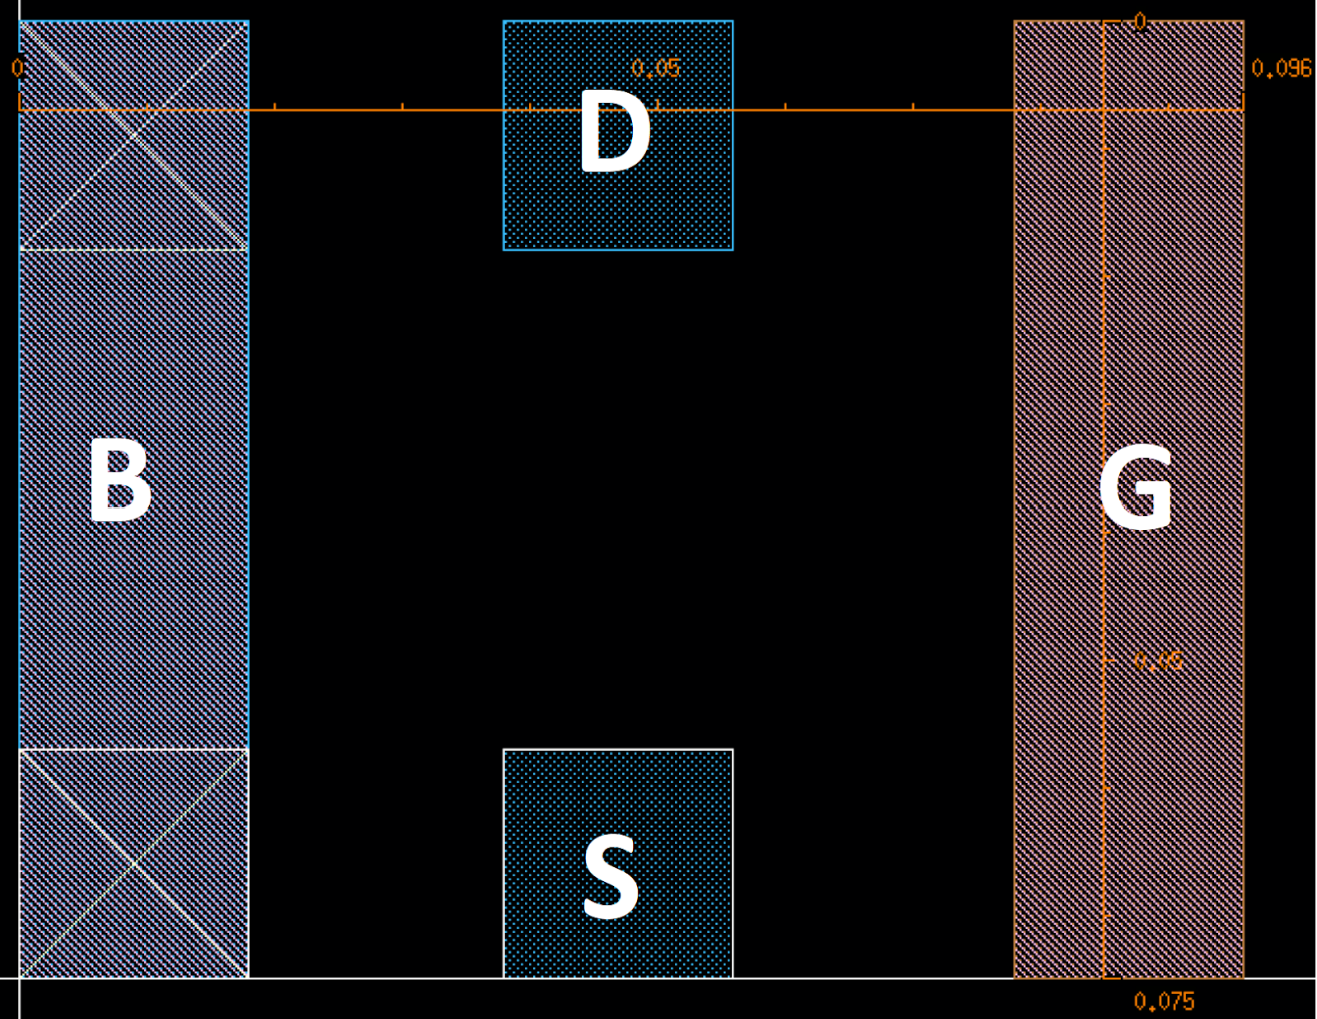
\includegraphics[width=0.5\textwidth]{figs/NEMlayout.png}
    \caption{Implemented NEM relay structure from M1 to M5}
    \label{fig:methods}
\end{figure}

% Detail final analysis that will be done
Area analysis is done using the Innovus post-PAR FPGA tile consisting of 4 connection blocks and a configurable logic block.
It is important to account for the additional metal area used by the relays, since they span M1-M5 and require routing to the half-select array. This should significantly impact the global place-and-route quality due to higher routing congestion. A .lef file was created to encode the relay layout and pinout information. Unfortunately, due to conflicts with hammer/ASAP7, the implemenation is prone to boundary DRC errors. This may partially be explained by the larger minimum metal widths in ASAP7 versus the published NEM relay this work was based on.

Power/timing analysis was also done in Innovus. For the NEM relays, a .lib file encoding the relay ON resistance and capacitance was created with ASAP7/Cadence Virtuoso.


%------------------------------------------------

%------------------------------------------------
% \section{Hypothesis}
% The vertical 4T relays should show a significant area reduction compared to the
% lateral relays reported in literature and CMOS-only FPGAs. However, due to the reduced routing resources caused
% by the use of additional metal layers in the vertical relays, we predict that the integrated
% performance results may counterbalance the benefits from the reduced lateral area. In both NEMS design 
% cases, we expect the area and performance to improve compared to the CMOS-only designs.
%------------------------------------------------

%------------------------------------------------
\section{Results}
The final layouts for the CMOS and NEMS FPGAs are shown in Figures \ref{fig:cmos}
and \ref{fig:NEMS} respectively. 

\begin{figure}[!hbt]
    \centering
    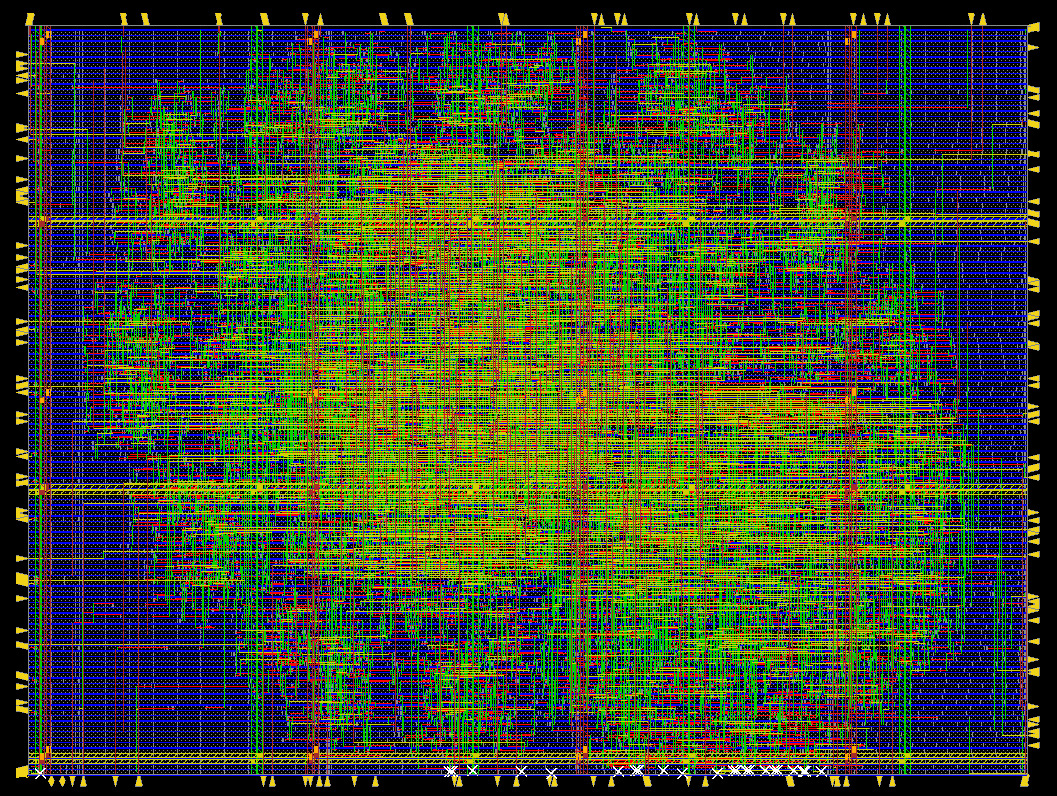
\includegraphics[width=0.3\textwidth]{figs/cmos_innovus.png}
    \caption{Post-PAR layout of CMOS FPGA}
    \label{fig:cmos}
\end{figure}

\begin{figure}[!hbt]
    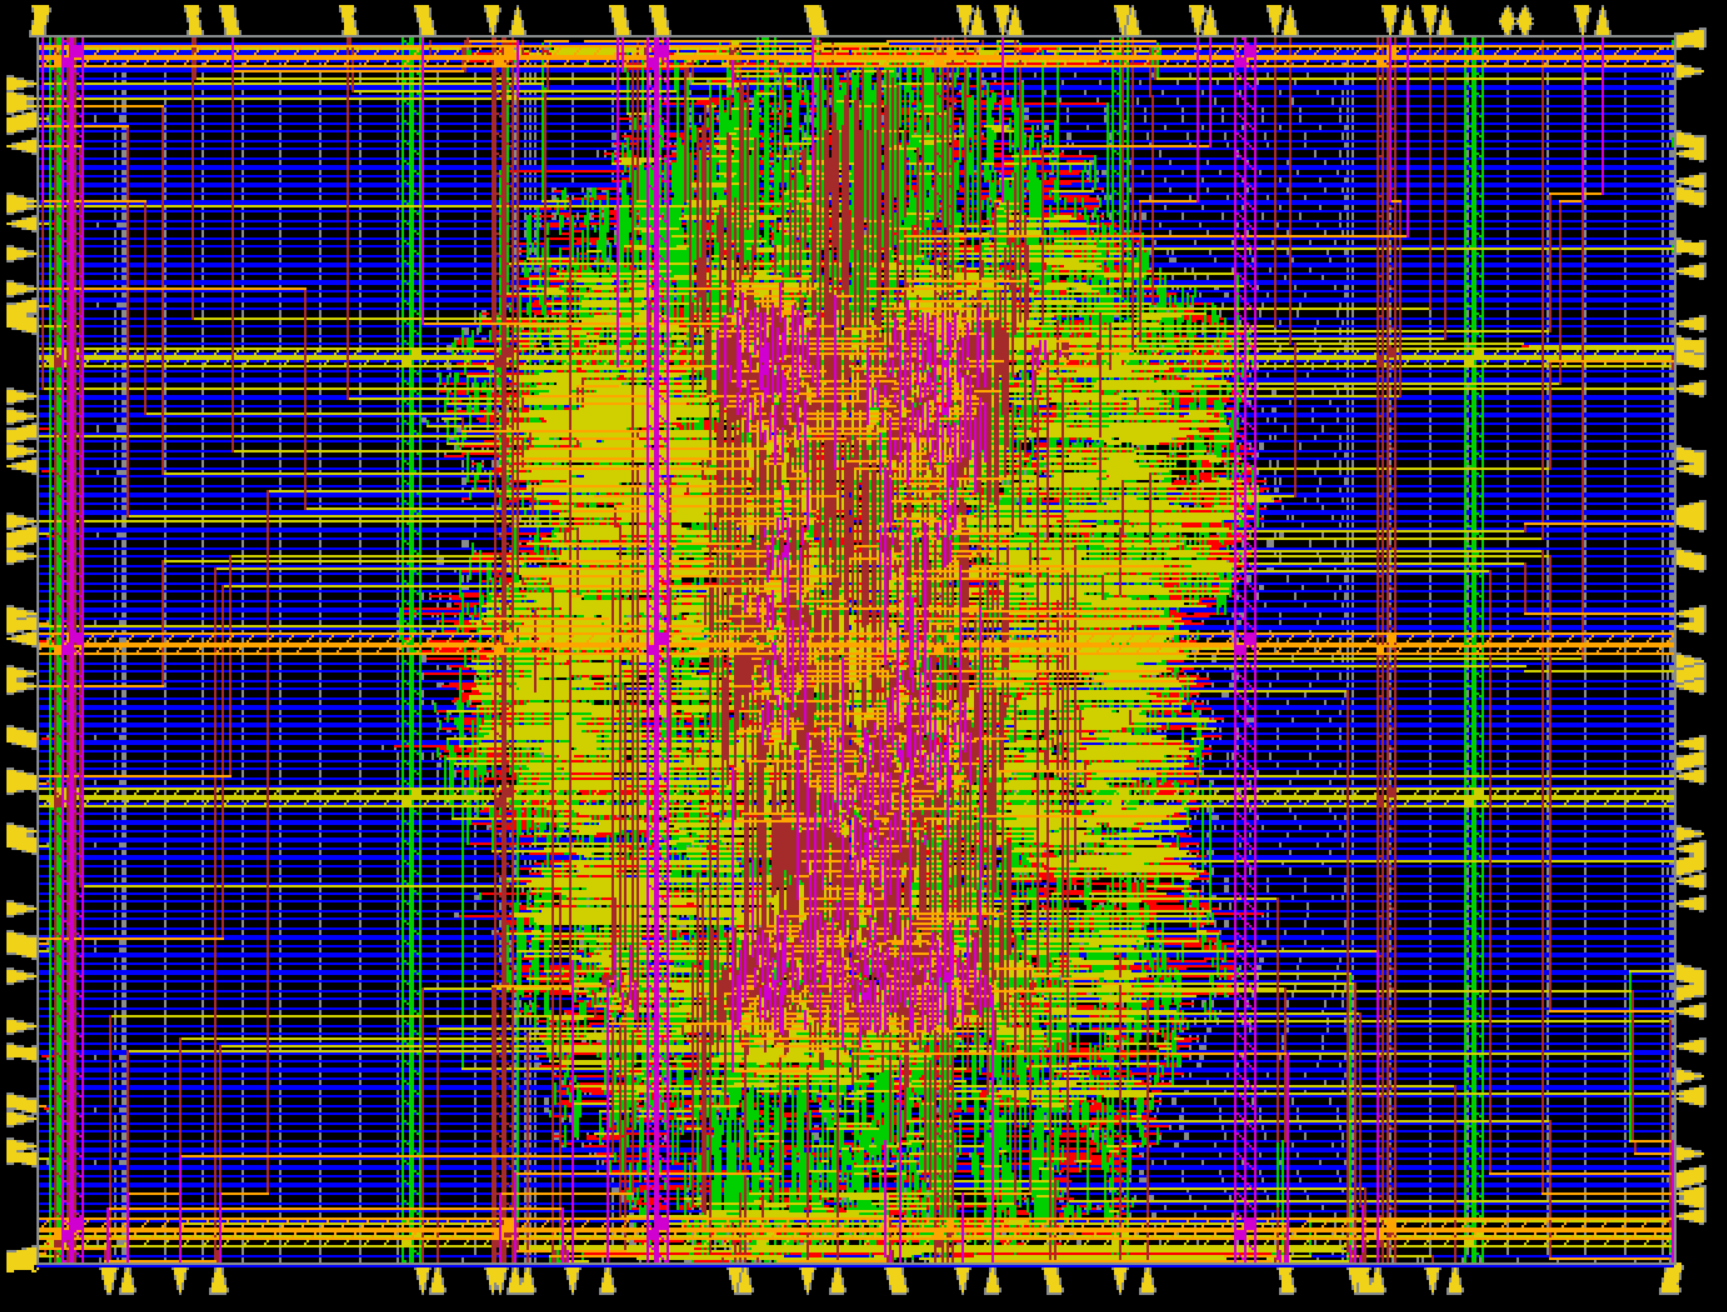
\includegraphics[width=0.3\textwidth]{figs/nems_innovus.png}
    \centering
    \caption{Post-PAR layout of NEMS FPGA}
    \label{fig:NEMS}    
\end{figure}

Fig. \ref{fig:area} shows the area for the different sub-blocks
for both the CMOS and NEMS based FPGAs. The included sub-blocks are the CLB,
\textit{blkinst}, and the four surrounding connection boxes: \textit{cbinstw}, 
\textit{cbinste}, \textit{cbinsts}, and \textit{cbinstn}. The CLB area remains 
nearly exactly the same; however, the size of all three CBs decreased by nearly 
100x. As discussed in Section \ref{sec:methods}, only the memory and switches
used for the connection boxes were replaced with NEMS relays and thus both 
results are expected and explainable. Further area reduction can be achieved
if the SRAM and muxes used inside the CLB block are also replaced with relays.
The total area reduction is $\approx 44\%$. 

\begin{figure}[!hbt]
    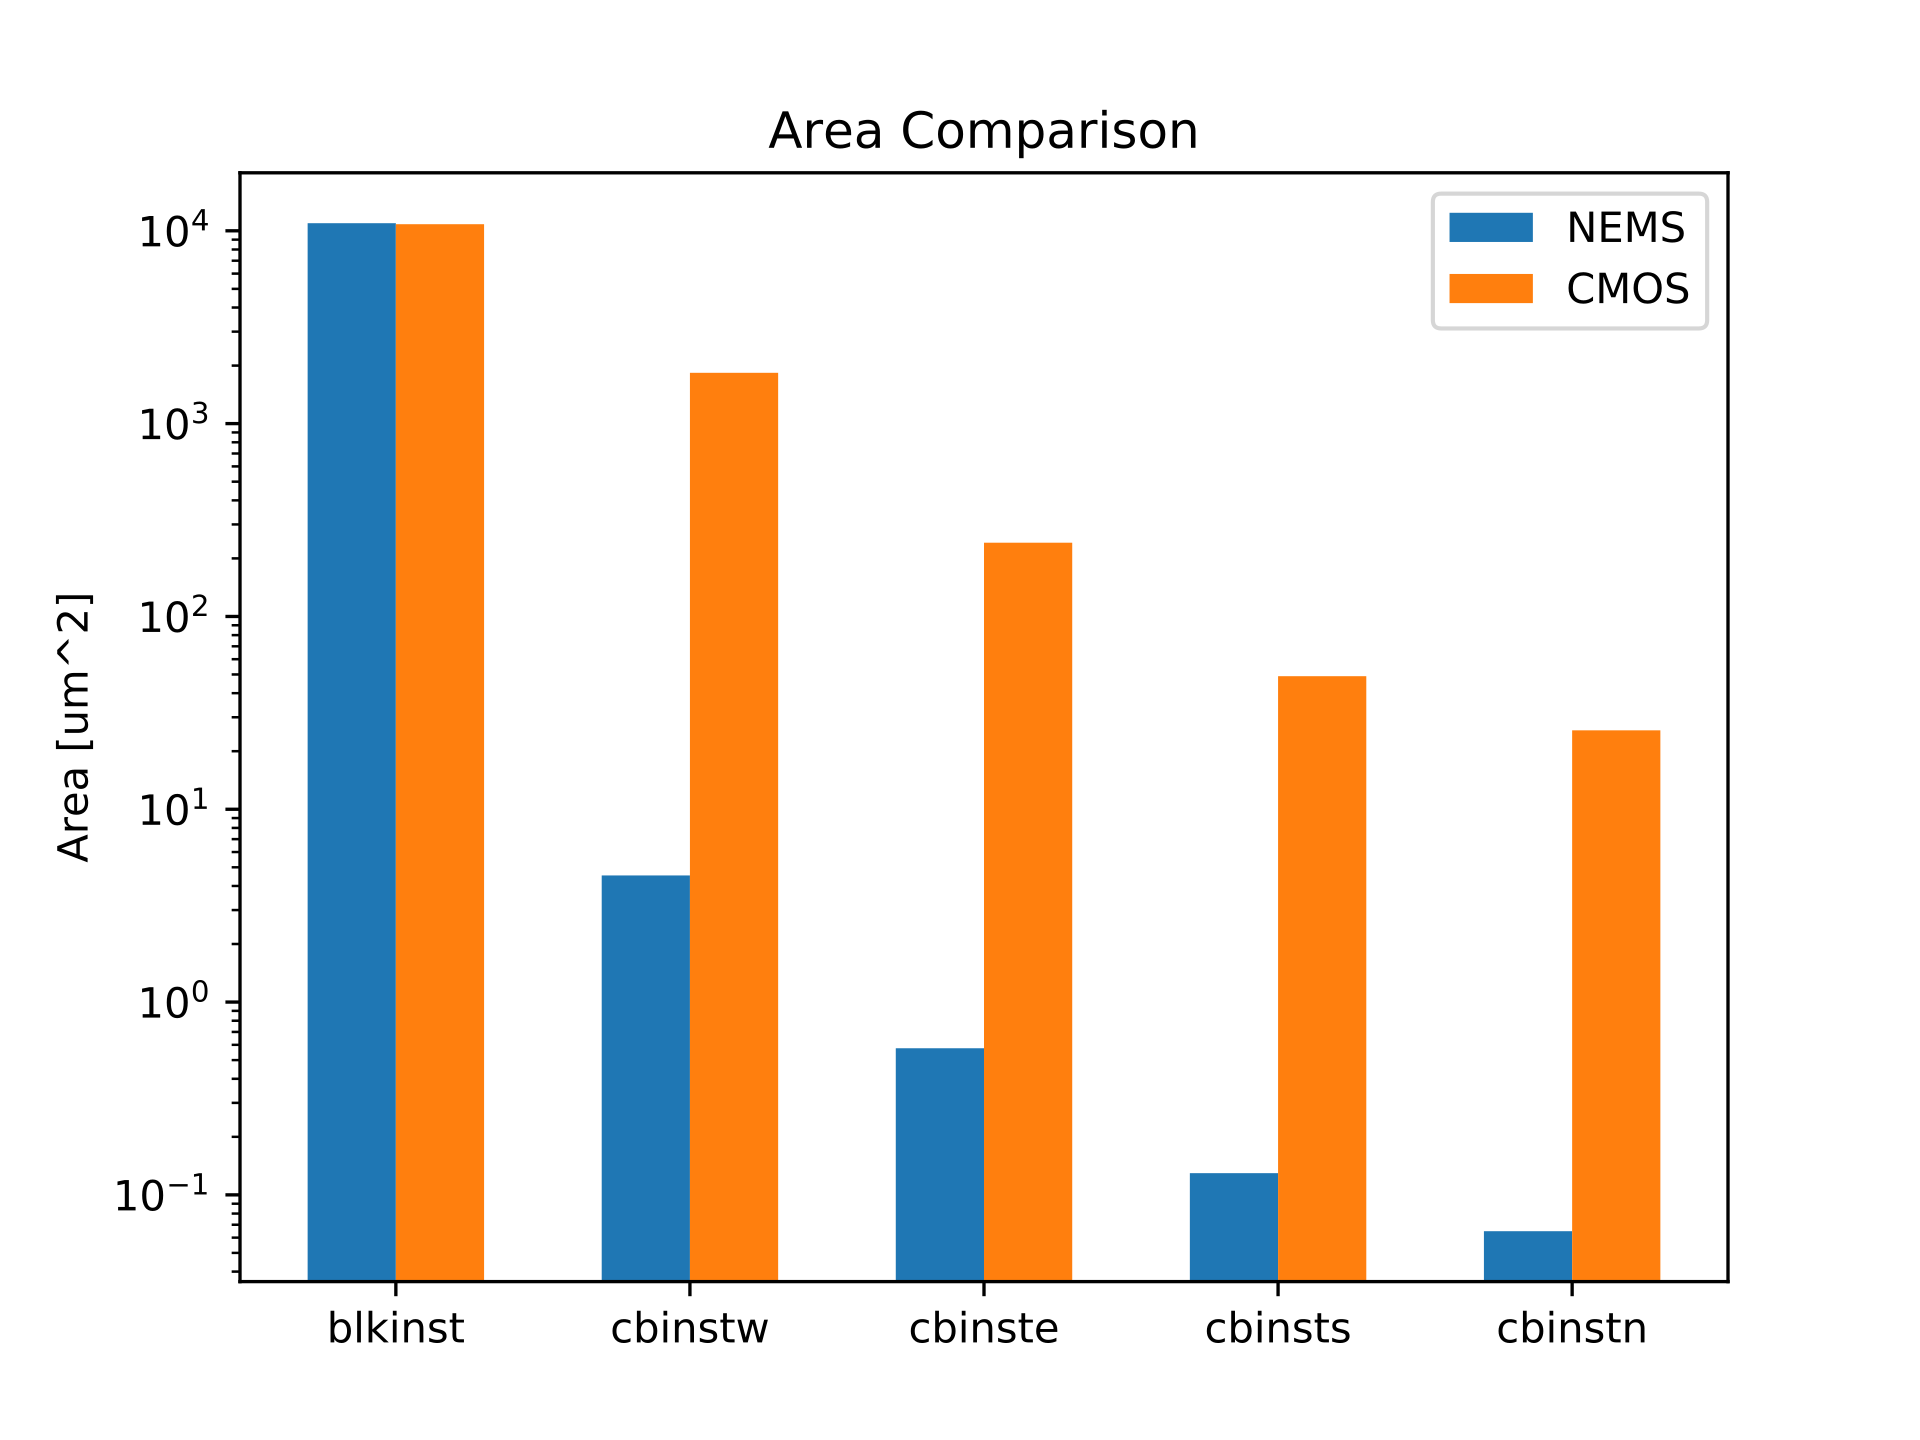
\includegraphics[width=0.5\textwidth]{figs/area_comparison.png}
    \centering
    \caption{Area comparison between NEMS and CMOS FPGA architectures}
    \label{fig:area}
\end{figure}

The static power reduction was around $48\%$ while the total power reduction
was around $22\%$. Reliable estimates for the dynamic power dissipation were 
not achieved for the NEMS relays and thus only the static power reduction numbers 
should be considered. However, we still expect the leakage power reduction to dominate 
the total power reduction, especially in this \SI{7}{\nano\meter} process. This is
supported by the fact that the CMOS FPGA's leakage power accounts for nearly $77\%$ 
of the total power while the NEMS FPGA's leakage accounts for nearly $71\%$.
%------------------------------------------------

%------------------------------------------------
\section{Conclusion}
We have reviewed several methods for creating BEOL NEMs relays in CMOS processes. 
Our proposed work will include the creation of 3 island-style FPGA tiles including NEMS 
supporting circuitry for direct comparison of area and performance between a traditional 
CMOS-only FPGA and two different styles of NEMS based FPGAs.

 Further analysis can be performed 
on the full FPGAs to determine the dissipated power and maximum 
operating frequency for each design for a given set of test circuits.
This will require connecting an array of FPGA tiles and running 
placement, packing, and routing to extract realistic performance and
utilization numbers. A popular open source tool known as the Verilog-to-Routing 
(VTR) project \cite{vtr8} can be used to perform this analysis.  


%----------------------------------------------------------------------------------------
%	REFERENCE LIST
%----------------------------------------------------------------------------------------

\printbibliography

%----------------------------------------------------------------------------------------

\end{document}
